\documentclass[a4paper,10pt]{scrartcl}

\input{pro6m_layout}


\begin{document}

\input{00_main/07_pro5m_main_titelpage}

% schrauben gewinde auf schraube anpassen
% Kristalltoleranzen sind massiv +-0.1
% Backe zwei sollte mit Durchgangsloch sein

% Was für einen strom hat der treiber übersteuerung(?)
% temp mit thermisotr misst temp. 18 und das muss geregelt werden. für diode und TEC.

% display mit sollwert und aktueller wert und evtl graphik wie stabil die temperatur ist

% steuerung/Regelung für TEC (abhängig der iode), Strom für Diode (treiber) welcher Storm/Spannung geeignet für dioden, kühlung für Diode
% 1 treiber für zwei TECs (aber hier für Diode und TEC)
% Welche Funktionalität für Die Steuerung für die Kiste
% Steuerung für den Alex-laser aufbauen und testen

% Personen Roamin Bla, Daniel Hug, *Philip Burger*

% wie mache ich die wasserkühlung

% kühlung über wasser oder über basisplatte

% optik: optische messungen pumpdiodenmodul faser biegung wie ändert sich der Polarisationstyp der faser abhängig der biegung
% polarisationskontroller (Ziel horizontale polarisation) 3 rollen (gleichung?)

% multimode mit mechanischer deformation überprüfen hands on mechanisch bewegung die
% dreht die polarisation, welche form? - linear, zirkular, elliptisch

% Diode, Faser, Powermeter leistung mit biegung

% wie gut bekommen wir es linear hin mit bewegung der faser
% dreht die biegung die polarisation und/oder verändert es sie auch

% infromieren what quarter- / halfwaveplate und polarizer are
% - Halfwaveplates:
%   Rotate Polarisation
% - Quarterwaveplates:
%   Turn linear to circular polarisation

% steuerung und Ausrichtung und evtl. polarisationstyp der wenn zeit ausreicht die kiste konzeptionel konstruieren

% diode mit tec und kristall mit tec

% für die pump diode TEC bestellen grösser

% Diode 29V und 550mA --> el. Leistung für diode

% Messung der Faser ca. 1Mnt.

% Steuerung

% Prototyp box

% https://optlasers.com/ --> Webseite des Treibers
\pagenumbering{arabic}
\section{Grundlagen}
Laser werden in der Wissenschaft oft zum Beispiel für die Messung und Untersuchung verschiedenster Proben im Mikrometerbereich, in der Medizin für Behandlungen und in der Industrie für die Bearbeitung von Materialien eingesetzt.\\
Um Laser für diese Anwendungen nutzen zu können, wird Licht in der Richtigen Wellenlänge bzw. deren Einstellbarkeit, Modi (CW oder gepulst) und Energiedichte benötigt. Zur Zeit werden oft unter anderen Titan-Saphir Laser eingesetzt, welche diese Eigenschaften gut vereinen, jedoch der Wirkungsgrad relativ niedrig ist.\\
Die Motivation einen mit roten Laserdioden gepumpten Alexandrit-Laser zu erforschen, liegt in der Leistungsausbeute dieser Laser. Die Leistungsausbeute ist mit dieser Kombination tendenziell höher, was die breite Anwendung in der Industrie und Wissenschaft attraktiv macht. Jedoch gibt es noch keinen im Femtosekunden-Bereich gepulster Alexandrit-Laser dieses Typs, die eine effiziente Applikation erlauben. Trotzdem haben sie das Potenzial die oben genannten Eigenschaften zu vereinen und noch zu übertreffen. Dazu kann der Alexandrit-Laser kompakter gebaut werden.\\

Damit ein Laser effizient betrieben werden kann, müssen die Bedingungen um den Laser gut sein. Dabei kommen unter Anderem der Temperatur des Kristalls und der Pumpdiode eine bedeutende Rolle zu. Daneben ist die Ausrichtung und die Polarisierung des Laserstrahls der Pumpdiode von grosser Wichtigkeit. Diese Parameter müssen eingestellt, geregelt und gesteuert werden, um einen gewünschten Arbeitspunkt zu erreichen.\\

\section{Aufgabenstellung}
Die Aufgabe in diesem Projekt (Pro6M) ist es,  die Steuerung für die Regelung der Temperatur des Kristalls und der Pumpdiode zu regeln. Für beide Komponenten werden TECs\footnote{en Thermo electric cooler, dt. Thermoelektrischer Kühler, auch Peltierelemente genannt.} eingesetzt (Abbildung \ref{fig:peltierelement}).  Die TECs werden über einen TEC-Kontroller (auch TEC-Treiber) geregelt. Dieser ist bereits in der Lage  die Parameter des PID-Reglers für die Temperaturen automatisch zu finden und einzustellen. Dies ermöglicht die Regelung der Temperaturen über Strom und Spannung. Die Diode sollte optimal bei 18°C gehalten werden, der Kristall bei 20°C.
Die Leistung der Pumpdiode soll separat mit einem Laserdioden-Treiber\footnote{LDD EN. Laser Diode Driver, dt. Laserdioden-Treiber} gesteuert werden können, dargestellt in Abbildung \ref{fig:ldd}. Dazu wird ein LDD mit in die Steuerung eingebaut. Dessen Stormstärke soll über einen analogen Eingang gesteuert werden indem manuell ein Wert der Steuerung übergeben wird.\\
Die Befehle für den TEC-Kontroller als auch für den Laserdioden-Treiber werden über einen Computer an die entsprechenden Komponente gesendet. Entsprechende Antworten der Komponenten werden wiederum in diesem Computer empfangen und verarbeitet. Dafür soll ein Raspberry PI Einplatinencomputer eingesetzt werden, gezeigt in Abbildung \ref{fig:raspberry_pi}.\\

Die gesamte Steuerung soll in einem Gehäuse untergebracht werden. Im Gehäuse sollen die Komponenten  (Raspberry PI, TEC-Kontroller, Laserdioden-Treiber, Digitalanzeige) intern mit Strom versorgt werden können. Dazu werden geeignete Netzteile für den Raspberry PI und ein Netzteil für den TEC-Kontroller bzw. dessen TECs und für den LDD mit in das Gehäuse eingebaut.\\
Die Funktionalität der gesamten Steuerung soll auf einem Testaufbau geprüft werden. Der Testaufbau soll für das Projekt mit den entsprechenden Komponenten aufgebaut werden.\\

Das übergeordnete Ziel der FHNW ist es, einen effizienten in Femtosekunden gepulsten Laser zu kreieren, der in der Industrie und der Wissenschaft und Froschung eingesetzt werden kann.\\
Ein entsprechender Aufbau eines Alexandrit-Lasers ist im Laserlabor der FHNW bereits vorhanden.\\

% Andererseits soll durch das Verändern der Form der Faser die Leistung des Oszillators optimiert werden.\\

\begin{figure}[H]
    \centering
    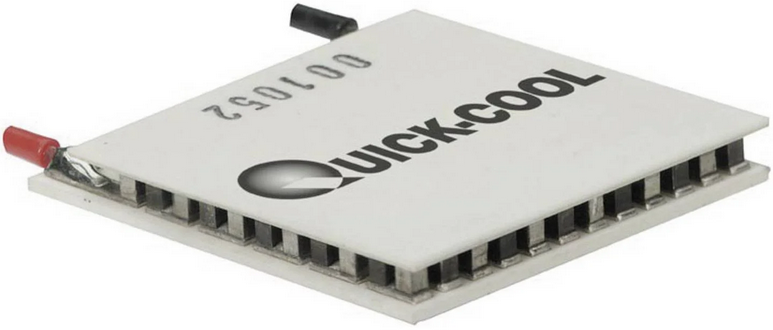
\includegraphics[scale=0.5]{10_images/peltier_modul.PNG}
    \caption{Abgebildet ist ein TEC der Marke Quick-Cool. Mit diesen elektrischen Bauteilen können bei Einspeisung von elektrischer Energie Kälte auf der Oberseite und Wärme auf der anderen Unterseite erzeugt werden. Wird die Richtung des Stromflusses geändert, vertauschen sich auch die warme und die kalte Seite.}
    \label{fig:peltierelement}
\end{figure}

\subsection{Regelung der TECs und des Laserdioden-Treibers}
Optimal sollen beide TECs mit einem einzigen Treiber mit zwei Kanälen geregelt werden können. Den Verlauf der Temperaturen soll bei Möglichkeit auf einer Digitalanzeige als Graphen abgebildet werden.

\begin{figure}[H]
    \centering
    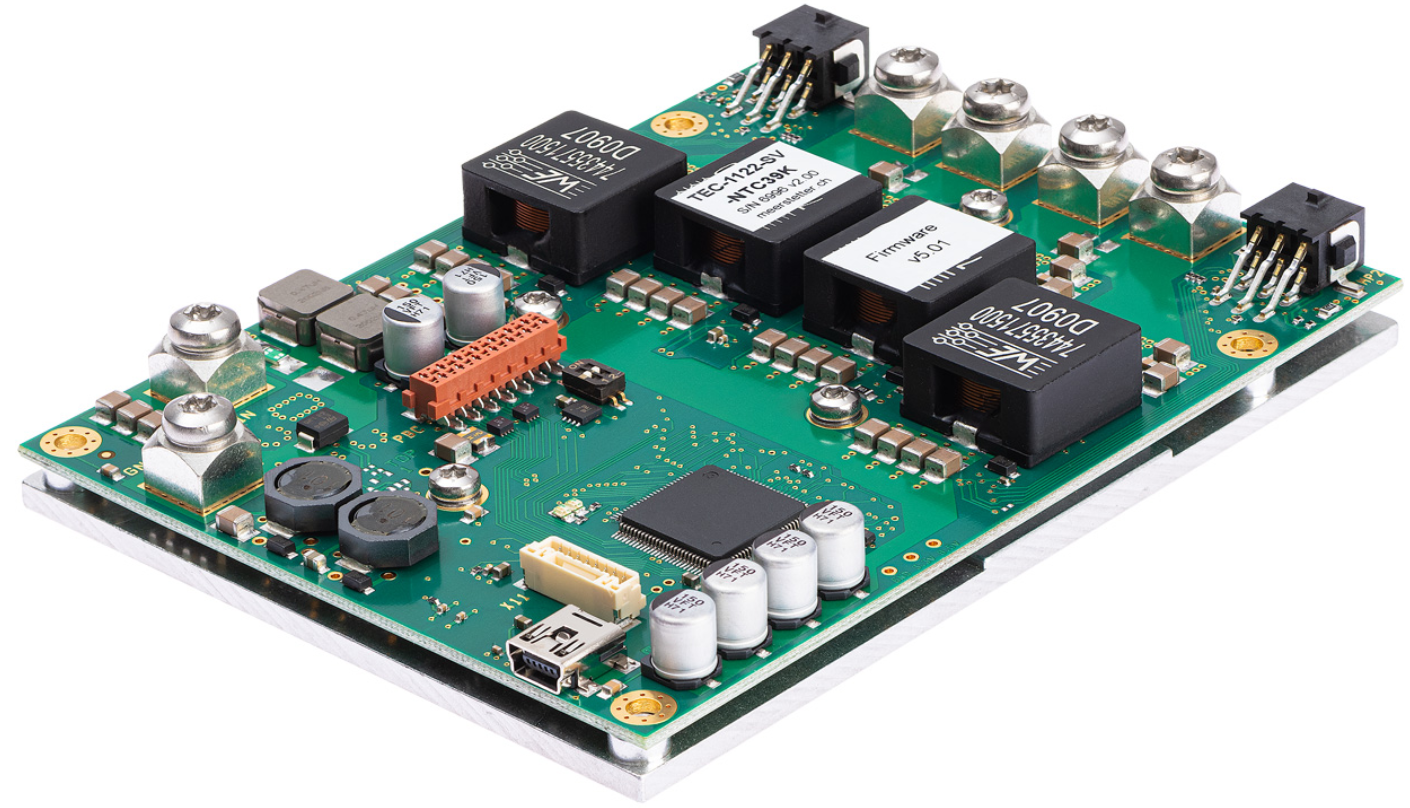
\includegraphics[scale=0.25]{10_images/tec_controller_real_isometry_meerstetter.PNG}
    \caption{Beispiel eines TEC-Treibers der Marke Meerstetter Engineering für die Steuerung der TECs. Die TECs werden direkt auf der Platine an den entsprechenden Ein- / Ausgänge angeschlossen. Abhängig vom Treibertyp, kann der Arbeitspunkt auch über die Potentiometer (P, I und D) auf der Platine manuell eingestellt werden.}
    \label{fig:tec_controller_free}
\end{figure}

Der Laserdioden-Treiber steuert die Stromzufuhr zur Pumpdiode. Dieser soll die Höhe des Stromflusses über die Steuerung erhalten. Der Stromfluss soll auf der Digitalanzeige manuell eingestellt werden können. Dafür muss eine Aus- und Eingangserweiternde Platine zum Raspberry PI angeschlossen werden, um auch analoge Signale verarbeiten zu können.
So kann der Laser ideal eingestellt werden. Die Leistung des Oszillators kann so gesteigert und durch die Steuerung die Handhabung des Lasers massiv vereinfacht werden.

\begin{figure}[H]
    \centering
%     %[trim={left bottom right top},clip]
    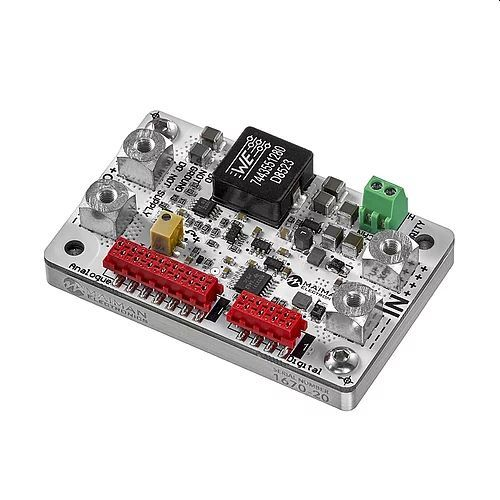
\includegraphics[scale=0.5, trim={0 30mm 0 40mm},clip]{10_images/SF6015.jpg}
    \caption{Beispiel eines Laserdioden-Treibers vom Hersteller Maiman. Dieser weist die Funktion auf den Stormfluss des Ausgangs über einen analogen Eingang steuern zu können.}
    \label{fig:ldd}
\end{figure}

\begin{figure}[H]
    \centering
    \includegraphics[scale=0.2]{10_images/Raspberry Pi-RASPBERRY PI 3 B-30085264-01.jpg}
    \caption{Beispiel eines Raspberry PI Einplatinencomputers vom Typ Raspberry PI 3B+ mit einer Arbeitsspannung von 5V. Dieser ist die Hauptkomponente und Steuert sowohl die TECs als auch den LDD und steuert die Digitalanzeige. Auf diesen wird die Platine mit den zusätzlichen Anschlüssen angeschlossen. Somit können alle weiteren Komponente Angeschlossen und gesteuert werden.}
    \label{fig:raspberry_pi}
\end{figure}

% \subsection{Optimierung der Ausgangsleistung des Oszillators durch Justieren der Faser}
% Die Ausgangsleistung des Oszillators wird stark durch die Art der Polarisation und deren Ausrichtung des Pumplasers beeinflusst. Dies hängt stark von der optischen Faser, in der der Pumplaser geleitet wird ab. Die Form der Glasfaser ist mechanisch so zu verändern, dass der ausgekoppelte Pumplaser eine möglichst optimale Form für den Oszillator aufweist. Herauszufinden ist, wie stark sich neben der Änderung der Ausrichtung der Polarisierung auch deren Form (linear, zirkular, elliptisch) verändert. Für die Anwendung in diesem Projekt wird eine möglichst horizontale und lineare Form angestrebt s. \ref{fig:polarization_forms_directions}.\\
% 
% \begin{figure}[H]
%     \centering
%     %[trim={left bottom right top},clip]
%     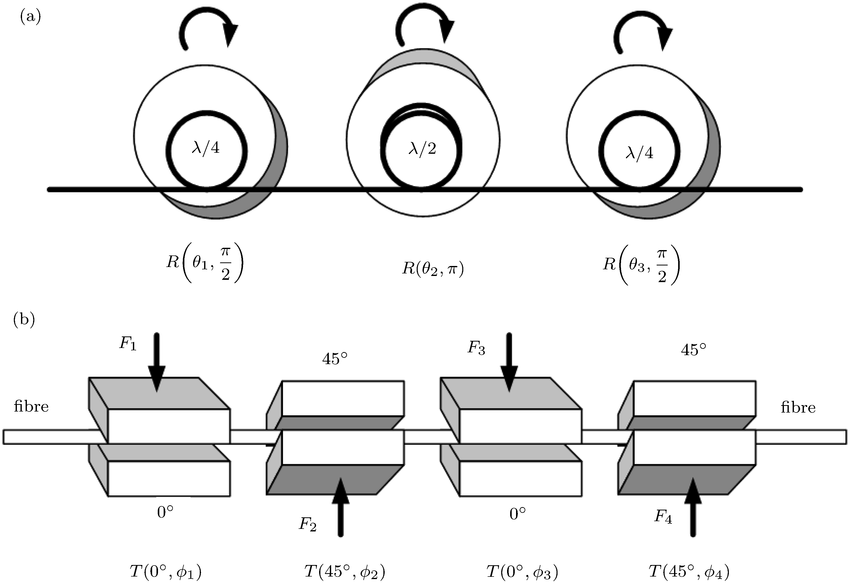
\includegraphics[scale=0.4, trim={15mm 125mm 0 0},clip]{10_images/laser_plarizationcontroller.png}
%     \caption{Beispiel eines Polarizationkontrollers für die Justierung der Glasfaser (Auf der Abbildung in fett-schwarz) für die Führung des Lasers in der Glasfaser.}
%     \label{fig:polarizationcontroller}
% \end{figure}
% 
% \begin{figure}[H]
%     \centering
%     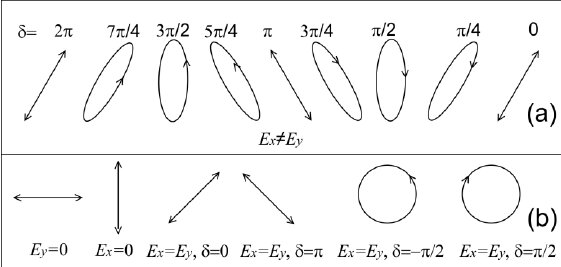
\includegraphics[scale=0.5, trim={5mm 10mm 0 14mm},clip]{10_images/laser_polarization_forms_directions.jpg}
%     \caption{Abgebildet sind verschiedene Formen und Ausrichtungen der Polarisation eines Laserstrahls in Richtung seiner Achse. Abgebildet sind lineare, elliptische und zirkulare Formen der Polarisation.}
%     \label{fig:polarization_forms_directions}
% \end{figure}
% 
% \subsection{Weiteres}
% Sollte der Zeitrahmen des Projektes dies erlauben, so ist die konzeptionelle Konstruktion des Gehäuses für den Laseraufbau zu erstellen.\\

\begin{landscape}
\includepdf[pages = 1, scale = 0.8, angle = 90, pagecommand={
\section{Zeitplan}
\subsection{Zeitplan}
\label{Variante B}}]
{02_pdfs/fhnw_pro6m_zeitplan_short_rev_4.pdf}

\includepdf[pages = 2, scale = 0.8, angle = 90, pagecommand={
\subsection{Zeitplan}
\label{Variante B}}]
{02_pdfs/fhnw_pro6m_zeitplan_short_rev_4.pdf}

\end{landscape}

\newpage
\includepdf[pages = 3, scale = 0.8, angle = 0, pagecommand={
\subsection{Zeitplan detailliert}
\label{Variante B}}]
{02_pdfs/fhnw_pro6m_zeitplan_short_rev_4.pdf}

\newpage
    \section{Ehrlichkeitserklärung}
Ich (wir) erkläre(n) hiermit, dass ich (wir) den vorliegenden Leistungsnachweis selber und selbständig verfasst habe(n),
\begin{itemize} 
\item dass ich (wir) sämtliche nicht von mir (uns) selber stammenden Textstellen und anderen Quellen wie Bilder etc. gemäss gängigen wissenschaftlichen Zitierregeln\footnote{z.B. APA oder IEEE} korrekt zitiert und die verwendeten Quellen klar sichtbar ausgewiesen habe(n); 
\item dass ich (wir) in einer Fussnote oder einem Hilfsmittelverzeichnis alle verwendeten Hilfsmittel (KI-Assistenzsysteme wie Chatbots\footnote{z.B. ChatGPT}, Übersetzungs-\footnote{z.B. Deepl} Paraphrasier-\footnote{z.B. Quillbot} oder Programmierapplikationen\footnote{z.B. Github Copilot}) deklariert und ihre Verwendung bei den entsprechenden Textstellen angegeben habe(n);
\item dass ich (wir) sämtliche immateriellen Rechte an von mir (uns) allfällig verwendeten Materialien wie Bilder oder Grafiken erworben habe(n) oder dass diese Materialien von mir (uns) selbst erstellt wurde(n);
\item dass das Thema, die Arbeit oder Teile davon nicht bei einem Leistungsnachweis eines anderen Moduls verwendet wurden, sofern dies nicht ausdrücklich mit der Dozentin oder dem Dozenten im Voraus vereinbart wurde und in der Arbeit ausgewiesen wird; 
\item dass ich mir (wir uns) bewusst bin (sind), dass meine (unsere) Arbeit auf Plagiate und auf Drittautorschaft menschlichen oder technischen Ursprungs (Künstliche Intelligenz) überprüft werden kann;
\item dass ich mir (wir uns) bewusst bin (sind), dass die Hochschule für Technik FHNW einen Verstoss gegen diese Eigenständigkeitserklärung bzw. die ihr zugrundeliegenden Studierendenpflichten der Studien- und Prüfungsordnung der Hochschule für Technik verfolgt und dass daraus disziplinarische Folgen (Verweis oder Ausschluss aus dem Studiengang) resultieren können.
\end{itemize}	\vspace{1cm}
	   Basel, den \today\\
	\vspace{1cm}
    	\begin{minipage}[t]{0.4\linewidth}
    		\textsf{Leroy Harreh}
    	   \begin{figure}[H]
                %[trim={left bottom right top},clip]
                
\includegraphics[scale=0.4, trim={0 0 10mm 0},clip]{10_images/unterschrift_leroy_harreh.PNG}
            \end{figure}
    		% \vspace{1.5cm}
    		\rule{6cm}{1px}
    		{\scriptsize  \hspace{2.7cm} Unterschrift}
    	\end{minipage}

        \vspace{1cm}

     	\begin{minipage}[t]{0.4\linewidth}
    		\textsf{Bojan Resan}
    	       \begin{figure}[H]
                % 
\includegraphics[scale=0.35]{10_images/unterschrift_leroy_harreh.PNG}
                \end{figure}
    		% \vspace{1.5cm}
    		\rule{6cm}{1px}
    		{\scriptsize  \hspace{2.7cm} Unterschrift}
    	\end{minipage}
\newpage

\end{document}